\documentclass[10pt]{article}          % the type of document and font size (default 10pt)
\usepackage[a4paper, tmargin=1.0in, bmargin=1.0in, lmargin=0.5in, rmargin=0.5in]{geometry}   
                                      % sets all margins to 1in, can be changed
\usepackage{moreverb}                 % for verbatimtabinput -- LaTeX environment
\usepackage{url}                      % for \url{} command
\usepackage{amssymb}                  % for many mathematical symbols
\usepackage[pdftex]{lscape}           % for landscaped tables
\usepackage{longtable}                % for tables that break over multiple pages
\usepackage[utf8]{inputenc}           % UTF8 characters
\usepackage[T1]{fontenc}
\usepackage{textcomp}
\usepackage[english]{babel}
\usepackage{float}                    % Position of figure, table
\usepackage{enumitem}                 % Alphabet list
\usepackage{makecell}                 % Customize cells in a table
\usepackage{amsmath}
\usepackage{amsfonts}
\usepackage{amssymb}
\usepackage{mathtools}
\usepackage{mathrsfs}
\usepackage{graphicx}
\usepackage{babel,blindtext}
\usepackage{ulem}
\usepackage{tabularx}
\usepackage[table]{xcolor}
\graphicspath{ {../output/} }
\DeclarePairedDelimiter{\ceil}{\lceil}{\rceil}
\renewcommand{\baselinestretch}{1.5}
\title{COCS 6323: Statistical Methods in Research \\ Group Project} % to specify title
\author{Group 2 \\
        Department of Computer Science\\
        University of Houston}         % to specify author(s)
\usepackage{Sweave}
\begin{document}                      % document begins here
\Sconcordance{concordance:ProjectReport.tex:ProjectReport.Rnw:%
1 31 1 1 0 13 1}
\Sconcordance{concordance:ProjectReport.tex:././sections/contribution2.Rnw:ofs 46:%
1 11 1}
\Sconcordance{concordance:ProjectReport.tex:ProjectReport.Rnw:ofs 58:%
47 2 1}
\Sconcordance{concordance:ProjectReport.tex:././sections/section4.Rnw:ofs 61:%
1 9 1}
\Sconcordance{concordance:ProjectReport.tex:ProjectReport.Rnw:ofs 71:%
51 2 1}
\Sconcordance{concordance:ProjectReport.tex:././sections/sectionT2.Rnw:ofs 74:%
1 32 1}
\Sconcordance{concordance:ProjectReport.tex:ProjectReport.Rnw:ofs 107:%
55 2 1}
\Sconcordance{concordance:ProjectReport.tex:././sections/sectionT3.Rnw:ofs 110:%
1 65 1}
\Sconcordance{concordance:ProjectReport.tex:ProjectReport.Rnw:ofs 176:%
59 4 1}


\setkeys{Gin}{width=1.0\textwidth}

\maketitle              % makes the title

\newpage
\tableofcontents        % inserts TOC (section, sub-section, etc numbers and titles)
\listoftables           % inserts LOT (numbers and captions)
\listoffigures          % inserts LOF (numbers and captions)

\newpage
\section{Contribution}
% !Rnw root = ../ProjectReport.Rnw
\begin{table}[h]
\begin{tabular}{|p{4cm}|p{13cm}|}
\hline
\textbf{Member} & \textbf{Contribution} \\ \hline
Bradley Macdonald & Analyze regression models of Figure 4\\ \hline
Tung Huynh & Preprocess Data, create and analyze regression models of Table S2, Table S3\\ \hline
Yifan Zhang & Preprocess Data, and draw plot of Figure 4 \\ \hline
\end{tabular}
\caption{Contribution of group members of the second milestone}
\label{tbl:contribution}
\end{table}

\newpage
\section{Figure 4}
% !Rnw root = ../ProjectReport.Rnw

\begin{figure}[!htb]
  \centering
  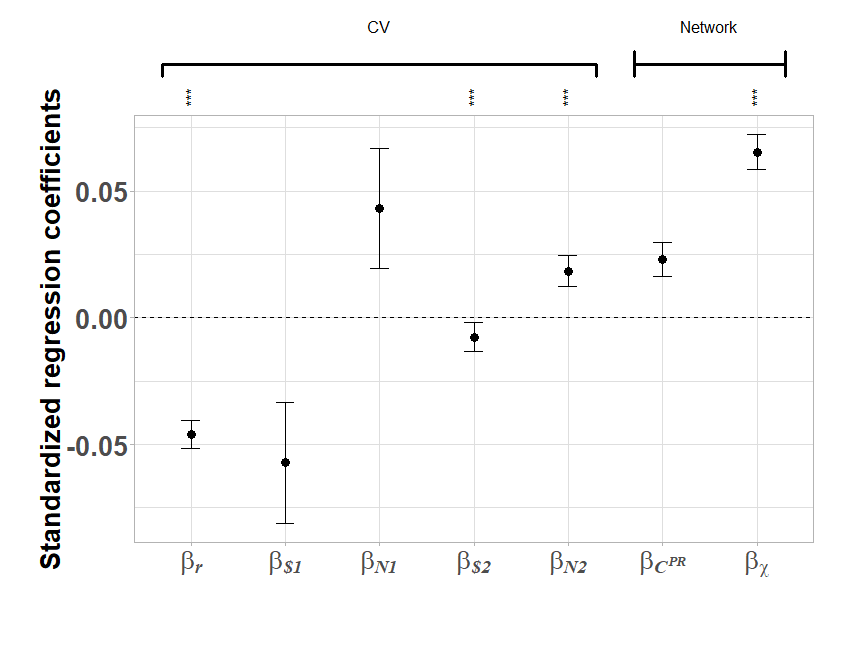
\includegraphics[width=12cm, height=10cm]{Figure4.png}
  \caption{Career cross-sectional regression model}
  \label{Fig4}
\end{figure}

Regression coefficients from Equation 1 were standardized and are presented with error bars indicating standard error. Prior to regression analysis, dummy variables were created for researcher discipline, as well as the five year period in which they published their first genomic publication. Zero's in the dataset (except for in dummy variables) were replaced by 0.00001 in order to allow for logarithmic transformations to be applied to appropriate numeric variables. The location which the information was derived from is indicated by the labels above the plot, with "CV" indicating the information was collected from the researcher's CV and "Network" indicating that the information originated from the researcher's collaboration network. Standardized beta coefficients are shown, to aid with the comparison across covariates. The plot shows the impact of changes in covariate, by showing the change in the dependant variable if the covariate were alterred by one standard deviation. "***" symbols were inserted above the covariates which showed statistical significance where the p-value was less than or equal to 0.001. The significant results indicate a covariate which impacts the dependant variable to a degree of statistical significance when alterred by one standard deviation.

\newpage
\section{Supplementary Table S2}
% !Rnw root = ../ProjectReport.Rnw
\hspace{0.5cm}This table shows the detail estimates for 3 models specified in Eq. (1). While in $CV$ models, 4,190 $F_i$ are taken into account to build the models, only 3,900 $F_i$ having network attributes, e.g. centrality, cross-disciplinary orientation, are used in the two $CV + Network$ models. In all models, most of the estimates have a significant confidence level except for the total amount of NSF $\beta_{\$1}$ fund and the number of NSF grants $\beta_{N1}$. In the $CV$ model, productivity index $\beta_{h}$ shows the most import impact on the increase of authors' citations. And even after removing 290 observation having not network attributes, its impact still keeps consistent and homogenous with a high confidence level. In the $CV + Network$ models, the positive value of $\beta_{\chi}$, the cross-disciplinary ratio ranging from 0.0 to 1.0, indicates the correlation with the career citations. With 0.1 elevation of $\chi$ correlates to 5.67\% increase in citations $C_i$. Therefore, the authors having greater $\chi_i$ will have a higher citation in the network.\\
\bigskip

\begin{table}[h]
\caption{Career data set: Poolel cross-sectional model}
\begin{tabular}{m{5cm} m{1.5cm} m{1.5cm} m{1.5cm} m{1.5cm} p{1.5cm} p{1.5cm} }
\\
\hline
\hline
& \multicolumn{2}{c}{\textbf{CV}} & \multicolumn{2}{c}{\textbf{CV + Network}} & \multicolumn{2}{c}{\textbf{CV + Network [Standardized]}} \\ \hline
\multicolumn{7}{l}{\textbf{CV parameters}} \\
{Department rank, $\beta_r$}          & -0.052***  & (0.006) & -0.047***  & (0.006) & -0.056***   & (0.007) \\
{Productivity ($h$-index), $\beta_h$} & 1.857***   & (0.018) & 1.866***   & (0.018) & 1.179***    & (0.012) \\
{Total NSF funding, $\beta_{\$1}$}    & -0.004*    & (0.002) & -0.005**   & (0.002) & -0.031**    & (0.012) \\
{\# of NSF grants , $\beta_{N1}$}     & 0.018      & (0.012) & 0.010      & (0.012) & 0.011       & (0.013) \\
{Total NIH funding, $\beta_{\$2}$}    & 0.015***   & (0.003) & 0.018***   & (0.003) & 0.072***    & (0.018) \\
{\# of NIH grants, $\beta_{N2}$}      & -0.062***  & (0.016) & -0.054**   & (0.017) & -0.060**    & (0.018) \\ \hline

\multicolumn{7}{l}{\textbf{Network parameters}} \\
{PageRank Centrality, $\beta_{\mathscr{C}^{PR}}$}   &  &            & 0.041**     & (0.014) & 0.026**   & (0.009) \\
{Cross-displinary, $\beta_{\chi}$}       &  &            & 0.567***    & (0.061) & 0.085***  & (0.009) \\ \hline

{Discipline ($\mathscr{O}$) dummy}                & Y &  & Y &  & Y &  \\
{5-year cohort ($y_{i,5^0}$) dummy}   & Y &  & Y &  & Y & \\
{Constant}                            & 1.400*** & (0.233) & 1.708*** & (0.271) & 7.743*** & (0.216) \\ \hline

{n}                                   & 4,190 &  & 3,900 &  & 3,900 & \\
{adj. $R^2$}                          & 0.883 &  & 0.882 &  & 0.882 & \\ \hline \hline
\multicolumn{7}{l}{\footnotesize{Standard errors in parentheses below estimate * p $\leq$ 0.05, ** p $\leq$ 0.01, *** p $\leq$ 0.0001}}

\end{tabular}
\label{tbl:sT2}
\end{table}


\newpage
\section{Supplementary Table S3}
% !Rnw root = ../ProjectReport.Rnw
\hspace{0.5cm}The below table displays the estimates values of variant models used to test the robustness of the cross-sectional model. In the first three variants, $Page Rank$, $Betweeness$ and $Degree$ are used as centrality measure alternatively. The authors having no centrality measure are eliminated from the model. In the fourth variant, the number of NSF grants and the number of NIH grants are eliminated due to the suspect of high correlation with the total amount of the corresponding fund. And in the last variant, the school rank is omitted from the model because this value only indicates the prominence effect of the school in recent years.

As extracted from the table, in all variants, the difference between the output estimate values from each model is not significant and even equal in some models. This test demonstrates the robustness of the cross-sectional model. In addition, high productivity index $\beta_h$ obviously has a high positive impact on the career of the authors.

In the variants (d) and (e), after removing variables of the number of grants and school rank correspondingly, the cross-sectional model still remains robust. This robustness proves the assumption that the number of grants having correlation effect with the total amount of fund and school rank does not indicate the success of authors' career accurately. 

Besides, while the estimates of the total amount of funds $\beta_{\$2}$ are positive correlate to the citations, the number of grants $\beta_{N2}$ has a negative correlation. This observation may be due to the effect of fund management.

\begin{table}[h]
\caption{Career data set: Poolel cross-sectional model - Robustness check}
\begin{tabular}{m{5cm} p{2.1cm} p{2.1cm} p{2.1cm} p{2.1cm} p{2.1cm} }
\\
\hline
\hline
& \textbf{(a)} & \textbf{(b)} & \textbf{(c)} & \textbf{(d)} & \textbf{(e)} \\
& {$\mathscr{C}^{PR}$} & {$\mathscr{C}^{B}$} & {$\mathscr{C}^{D}$} & \sout{$\beta_{N1}, \beta_{N2}$} & \sout{$\beta_{r}$} \\ \hline

\multicolumn{6}{l}{\textbf{CV parameters}} \\
\rowcolor{lightgray}
{Department rank, $\beta_r$}          & -0.047*** & -0.042*** & -0.044*** & -0.046*** &           \\
                                      & (0.006)   & (0.006)   & (0.006)   & (0.006)   &           \\
\rowcolor{lightgray}                               
{Productivity ($h$-index), $\beta_h$} & 1.866***  & 1.901***  & 1.848***  & 1.862***  & 1.892***  \\
                                      & (0.018)   & (0.019)   & (0.018)   & (0.018)   & (0.018)   \\
\rowcolor{lightgray}
{Total NSF funding, $\beta_{\$1}$}    & -0.005**  & -0.004*   & -0.004*   & -0.003**  & -0.004*   \\
                                      & (0.002)   & (0.002)   & (0.002)   & (0.001)   & (0.002)   \\
\rowcolor{lightgray}
{\# of NSF grants , $\beta_{N1}$}     & 0.010     & 0.009     & 0.005     &           & 0.004     \\
                                      & (0.012)   & (0.012)   & (0.012)   &           & (0.012)   \\
\rowcolor{lightgray}
{Total NIH funding, $\beta_{\$2}$}    & 0.018***  & 0.012***  & 0.012***  & 0.003*    & 0.012***  \\
                                      & (0.003)   & (0.003)   & (0.003)   & (0.001)   & (0.003)   \\
\rowcolor{lightgray}
{\# of NIH grants, $\beta_{N2}$}      & -0.054**  & -0.056**  & -0.055**  &           & -0.052**  \\
                                      & (0.017)   & (0.017)   & (0.017)   &           & (0.017)   \\ \hline

\multicolumn{6}{l}{\textbf{Network parameters}} \\
\rowcolor{lightgray}
{PageRank Centrality, $\beta_{\mathscr{C}^{PR}}$}     & 0.041** &  &              & 0.042**   & 0.057***  \\ 
                                              & (0.014) &  &              & (0.014)   & (0.014)   \\
\rowcolor{lightgray}
{Betweeness Centrality, $\beta_{\mathscr{C}^B}$}    &  & -0.0003 &  &  &  \\ 
                                              &  & (0.005) & & & \\
\rowcolor{lightgray}
{Degree Centrality, $\beta_{\mathscr{C}^D}$}        &  &  & 0.052*** & & \\ 
                                              &  &  & (0.010) & & \\
\rowcolor{lightgray}
{Cross-displinary, $\beta_{\chi}$}          & 0.567***  & 0.560***  & 0.526***  & 0.579***  & 0.552***  \\
                                            & (0.061)   & (0.062)   & (0.061)   & (0.061)   & (0.061) \\ \hline

\rowcolor{lightgray}
{Discipline ($\mathscr{O}$) dummy}                & Y & Y & Y & Y & Y  \\
\rowcolor{lightgray}
{5-year cohort ($y_{i,5^0}$) dummy}   & Y & Y & Y & Y & Y \\
\rowcolor{lightgray}
{Constant}                            & 1.708***  & 1.204***  & 1.345***  & 1.711***  & 1.617***  \\ 
                                      & (0.271)   & (0.225)   & (0.226)   & (0.270)   & (0.272)   \\ \hline

\rowcolor{lightgray}
{n}                                   & 3,900 & 3,387 & 3,900 & 3,900 & 3,900 \\
\rowcolor{lightgray}
{adj. $R^2$}                          & 0.882 & 0.873 & 0.883 & 0.882 & 0.881 \\ \hline \hline
\multicolumn{6}{l}{\footnotesize{Standard errors in parentheses below estimate * p $\leq$ 0.05, ** p $\leq$ 0.01, *** p $\leq$ 0.0001}}

\end{tabular}
\label{tbl:sT3}
\end{table}

\bigskip   % leave some empty space (optional)

\end{document}

